\chapter{$p$-$n$ Junction Diode}\label{chap1}

The term diode\index{Diode} denotes a two electrode device. {\bf Di} means {\bf two} and {\bf ode} means electrode. A semiconductor diode is a two layer single junction two terminal unidirectional device. The current in a diode is contributed by both holes and electrons. Diode is the simplest of all semiconductor devices but plays a very important role in electronic systems. Diodes are used in variety of applications including communication systems, radio, TV, computers, power supplies and so on.  
This chapter begins with an explanation of the $p$-$n$ junction diode
and proceeds with its characteristics and parameters. Diode
approximations, dc and ac equivalent circuits, temperature effects are
presented with numerous examples. Zener diode and its characteristic have also been discussed at the end of this chapter.

\section{{\boldmath$p$-$n$} junction}\label{sec1.1}
\index{pn@$p{\rm-}n$ junction}

A $p$-$n$ junction diode is a two terminal unidirectional device with
a $p$-type anode and an $n$-type cathode as shown in Fig. 1.1. It is
said to be forward biased when its anode is kept at a positive
potential with respect to its cathode. Under this condition, it
offers a low resistance to the flow of current and acts as the closed
condition of a switch. The current flowing in this condition is called
forward current,\index{Forward current} $I_F$.
\begin{figure}[H]
\centering
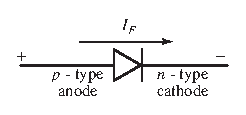
\includegraphics[scale=1.25]{chap1/S3-EE-01-001.eps}
\caption{Forward biased $p$-$n$ junction diode}\label{fig1.1}
\end{figure}

\eject

It is said to be reverse biased when its anode is kept at a negative
potential with respect to its cathode is shown in Fig. 1.2. It now
offers a very high resistance to the flow of current and acts as the
open condition of a switch. The current flowing in this condition is
called reverse current\index{Reverse current} $I_R$.
\begin{figure}[H]
\centering
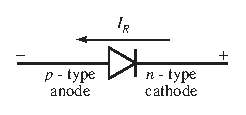
\includegraphics[scale=1.25]{chap1/S3-EE-01-002.eps}
\caption{Reverse biased $p$-$n$ junction diode}\label{fig1.2}
\end{figure}

It is clear that 
\begin{equation}
|\,I_F\,| \gg |\,I_R\,| \label{eq1.1}
\end{equation}


\section{Conditions under which a {\boldmath$p$-$n$} junction diode
  can be destroyed}\label{sec1.2}
The diode can be destroyed when 
\begin{itemize}
\item It is over heated by a high forward current flowing
  through the diode. Power dissipation is given by
\begin{equation}
P = I^2_F\, R_F \label{eq1.2}
\end{equation}
where $I_F$ is the forward current in the diode and $R_F$ is the
resistance of the diode when forward biased.

\item A large reverse voltage causes the $p$-$n$ junction to
  break down.\index{Break down}
\end{itemize}

Thus the maximum forward current $I_{F(\max)}$ and the maximum reverse
voltage $V_{R(\max)}$ are important specifications given in the
diode manufacturer's data sheets. It can also be observed that
physically larger diodes can pass large currents and withstand large
reverse voltage while smaller diodes are limited to small forward
current and reverse voltages.

\section{Classification of diodes based on currents}\label{sec1.3}
\index{Diode!classification}

Based on currents, diodes may be classified as:
\begin{itemize}
\itemsep=1pt
\item low-current diodes
\item medium-current diodes
\item high-current diodes
\end{itemize}

\section{Description and ratings of a low-current diode}\label{sec1.4}

Typically low-current\index{Diode!low-current} diodes have a body 3 mm long with a coloured
band close to the cathode for identification as shown in Fig. 1.3.
\begin{figure}[H]
\centering
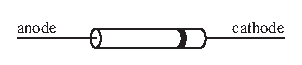
\includegraphics[scale=1.2]{chap1/S3-EE-01-003.eps}
\caption{Low-current diode}\label{fig1.3}
\end{figure}


These diodes can withstand forward currents of the order of 100 mA and
reverse voltages of about 75 V. The reverse current at room
temperature is typically less than $1\mu A$.

\section{Description and ratings of a medium-current diode}\label{sec1.5}

Medium current\index{Diode!medium current} diodes are packaged in a metal can-like casing of
typical diameter 8.9 mm and length 7.6 mm as shown in Fig. 1.4.
\begin{figure}[H]
\centering
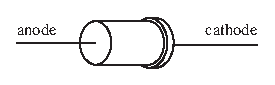
\includegraphics[scale=1.2]{chap1/S3-EE-01-004.eps}
\caption{Medium current diode}\label{fig1.4}
\end{figure}

They can carry a forward current in the range of about 400-500 mA and
withstand reverse voltages of about 200-300 V.

\section{Description and ratings of high-current diode}\label{sec1.6}

The appearance of a high-current\index{Diode!high-current} diode in a solid metal package is
shown in Fig. 1.5
\begin{figure}[H]
\centering
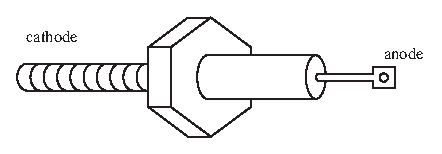
\includegraphics[scale=1.15]{chap1/S3-EE-01-005.eps}
\caption{High-current diode}\label{fig1.5}
\end{figure}

The diode is screwed onto a metal heat sink for quick dissipation of
the heat generated when high current is conducted through the
device. Typical body diameter is 7.8 mm and the total length is 31.2
mm. These diodes can carry several amperes of current and can
withstand several hundred of volts in reverse bias.\\[-20pt]

\section{Forward and reverse characteristics of a Silicon diode}\label{sec1.7}
\index{Diode!silicon}

A diode conducts a large forward current, $I_F$ when forward biased
with its anode at a positive potential with respect to its cathode. It
conducts a comparatively much smaller reverse current, $I_R$ when
reverse biased with its anode at a negative potential with respect to
its cathode. This behaviour can be illustrated in the forward and
reverse characteristics shown in Fig. 1.6.
\begin{figure}[H]
\centering
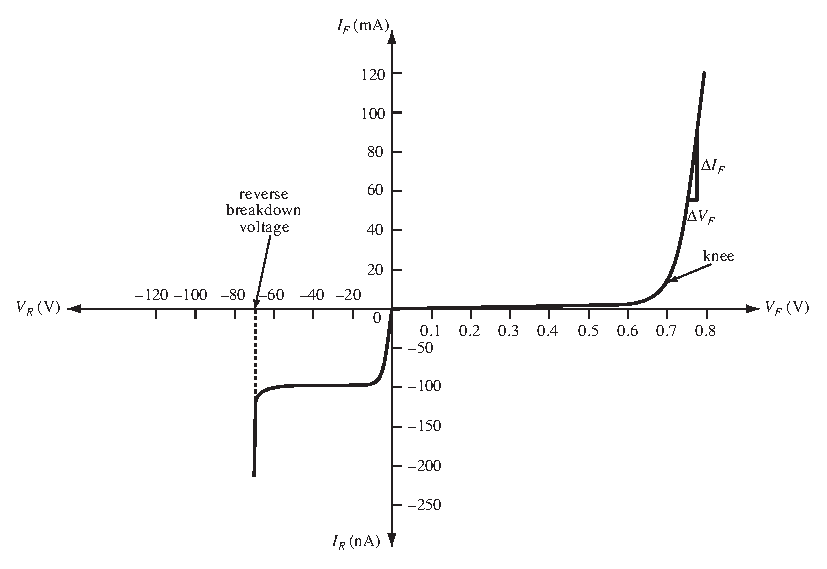
\includegraphics[scale=.9]{chap1/S3-EE-01-006.eps}
\caption{Characteristics of a Silicon diode}\label{fig1.6}
\end{figure}

\heading{Forward characteristics}\index{Forward characteristics}
\begin{itemize}
\itemsep=1pt
\item[$\bullet$] For forward bias voltages less than 0.7\,V, the forward current, $I_{F}$, remains very low.

\item[$\bullet$] When the forward bias voltage, $V_{F}$, exceeds 0.7\,V, the current rapidly increases and the diode is to be {\em on}.

\item[$\bullet$] In this region a small change in forward voltage, $\Delta V_{F}$, causes a large change in forward current $\Delta I_{F}$.

\item[$\bullet$] The voltage at which the diode begins to conduct the forward current appreciably is called the cut-in voltage, denoted by $V_{\gamma}$. As indicated in Fig.~\ref{fig1.6}, $V_{\gamma}$ is about 0.7\,V for silicon diode.\\[-18pt]
\end{itemize}

\heading{Reverse Characteristics}\index{Reverse characteristics}
\begin{itemize}
\itemsep=1pt
\item[$\bullet$] For small reverse voltages, the reverse current $I_{R}$, through the diode is very small, typically less than 100\,nA.

\item[$\bullet$] When the reverse bias voltage exceeds breakdown voltage, the current through the diode increases sharply. As such from the graph, the reverse breakdown voltage is around 75\,V, for the diode under consideration. 

\item[$\bullet$] Reverse breakdown\index{Reverse breakdown} is a destructive phenomena. Hence for safe operation the applied reverse voltage should not exceed the breakdown voltage.

\item[$\bullet$] Observe from the graph that, $|\,I_{R}\,|\ll |\,I_{F}\,|$. Also the diode is said to be {\em off}, under reverse bias and also for forward voltages less than $V_{\gamma}$, since the diode current is almost zero.
\end{itemize}


\begin{example}\label{exam1.1}
Find the forward and reverse resistance at $I_F = 100\mA$ and $V_R = 25
V$ respectively for the silicon diode whose characteristics is shown
in below. What is the cut-in voltage?
\begin{figure}[H]
\centering
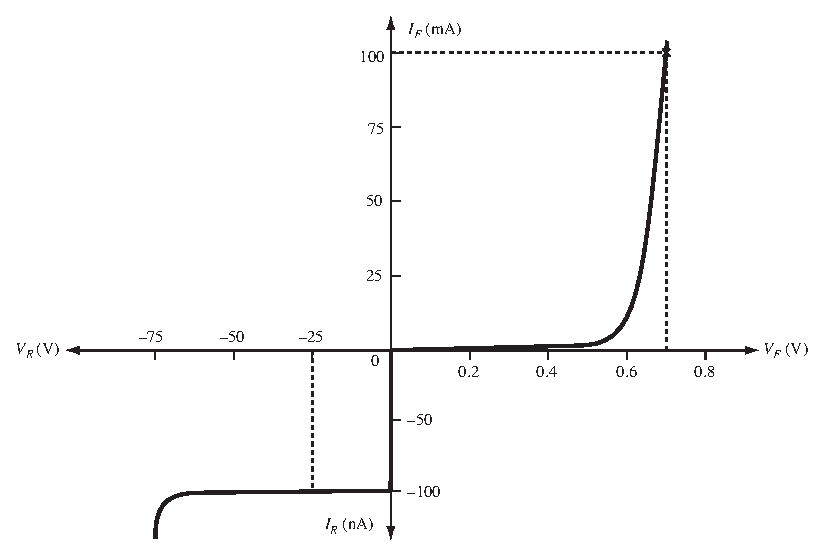
\includegraphics{chap1/S3-EE-01-007.eps}
%\caption{}\label{fig1.7}
\end{figure}
\end{example}

\eject

\begin{solution}
Given, $I_F = 100 \mA$

From the characteristics given in Figure, $V_F = 0.7V$ at $I_F = 100
\mA$.

We know that resistance is the ratio of voltage and current.

Hence, forward resistance $R_F$ is given by
\begin{align*}
R_F & = \frac{V_F}{I_F}\\[5pt]
& = \frac{0.7V}{100~ \mA}\\[5pt]
& = \frac{0.7 V}{0.1 A} = 7 \Omega
\end{align*}

The diode forward resistance is normally represented as either $R_F$
or $R_f$. Both these forms are used in this text. It is the resistance
of a diode when it is {\it on}. $R_F$ is referred to as the static
forward resistance. Now, given 
$$
V_R = 25 V,
$$
again from the given characterstics $I_R = 100$ nA at $V_R = 25~ V$.

Hence the static reverse resistance $R_R$ is given by, 
\begin{align*}
R_R & = \frac{V_R}{I_R}\\[5pt]
& = \frac{25 V}{100\text{\,nA}}\\[5pt]
& = \frac{25 V}{0.1 \mu A} = 250 M \Omega
\end{align*}

It is the resistance of the diode when it is {\it off}.

Note that 
$$
I_R \ll I_F \quad \text{ and }\quad  R_R \gg R_F
$$

Thus the diode offers high resistance when reverse biased or {\it off}
and low resistance when forward biased or on. 

From the knee of the characteristics we can say that the cut-in
voltage, $V_\gamma$ is approximately 0.6V.
\end{solution}

\eject

\begin{example}\label{exam1.2}
Find the static forward resistance at 200 mA for the diode whose
characteristics is shown below. Also find the reverse resistance at a
reverse voltage of 75 V.
\begin{figure}[H]
\centering
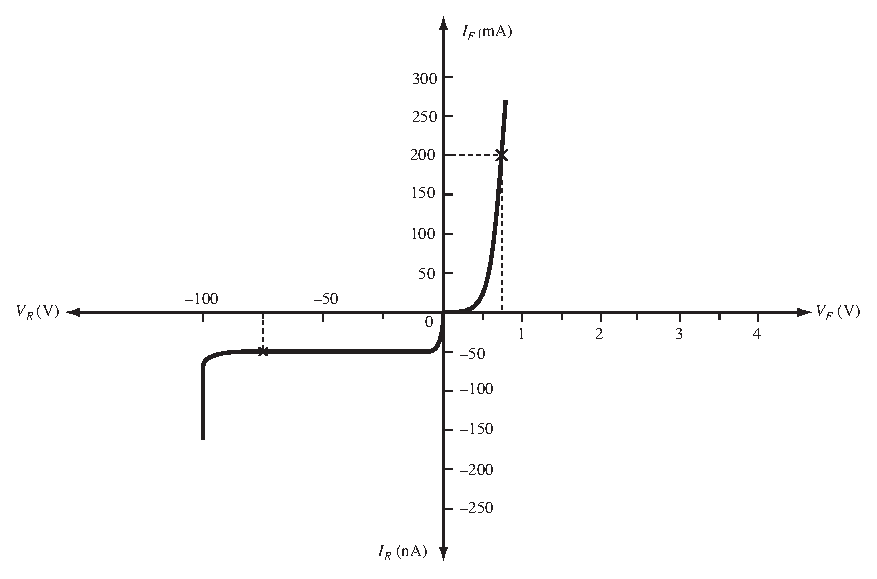
\includegraphics{chap1/S3-EE-01-008.eps}
%\caption{}\label{fig1.7}
\end{figure}
\end{example}

\begin{solution}
Given, $I_F = 200\mA$

From the characteristics given in Figure 

at $I_F = 200\mA$, $V_F =0.75$ V

$\therefore$ By definition, static forward resistance, 
$$
R_F = \frac{V_F}{I_F} = \frac{0.75 V}{200 \mA} = \frac{0.75 V}{0.2 A} =
3.75 \Omega
$$

Given, $V_R = 75 V$

From the characteristics, 

At $V_R =75V$, $I_R = 50~ nA$

$\therefore$ By definition, the static reverse resistace,
$$
R_R = \frac{V_R}{I_R} = \frac{75 V}{50 nA} = \frac{75 V}{0.05 \mu A} =
150 M \Omega
$$

Note that $R_F \ll R_R$ as expected.
\end{solution}


\section{Forward and reverse characteristic of a Germanium diode}\label{sec1.8}

Fig.~\ref{fig1.7} shows the forward and reverse characteristics of Germanium\index{Diode!germanium} diode.
\begin{figure}[H]
\centering
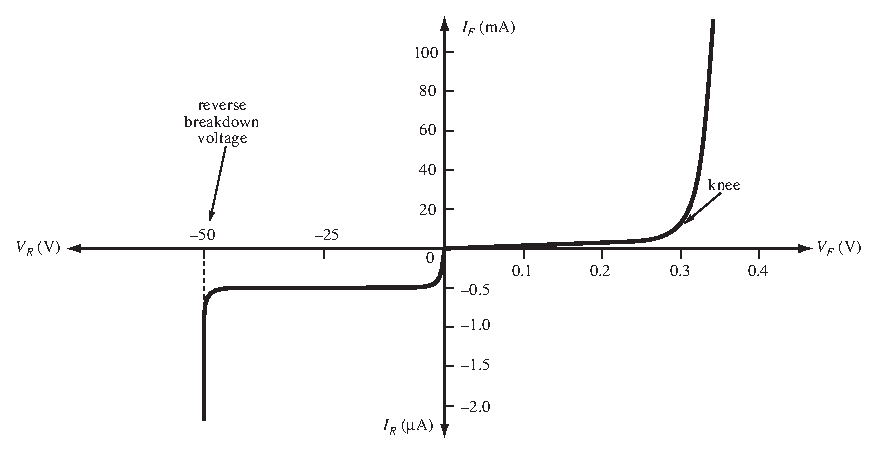
\includegraphics{chap1/S3-EE-01-009.eps}
\caption{Characteristics of Germanium diode}\label{fig1.7}
\end{figure}

\heading{Forward characteristics}\index{Forward characteristics}
\begin{itemize}
\item[$\bullet$] The diode is said be forward biased when its anode potential is positive with respect to its cathode potential.

\item[$\bullet$] For forward bias voltages less than 0.3\,V, the forward current $I_{F}$ remains very low.

\item[$\bullet$] When the forward bias voltage $V_{F}$ exceeds 0.3\,V, the forward current rapidly increases and the diode is said to be {\em on}.

\item[$\bullet$] In this region a small change in forward voltage, $\Delta V_{F}$, causes a large change in forward current, $\Delta I_{F}$.

\item[$\bullet$] The voltage at which the diode begins to conduct the forward current appreciably is called the cut-in voltage, denoted by $V_{\gamma}$. As indicated in Fig.~\ref{fig1.7}, $V_{\gamma}$ is about 0.3\,V for germanium diode.
\end{itemize}

\eject

\heading{Reverse characteristics}\index{Reverse characteristics}
\begin{itemize}
\item[$\bullet$] The diode is said to be reverse biased when its anode potential is negative with respect to its cathode potential.

\item[$\bullet$] For small reverse voltages, the reverse current $I_{R}$ through the diode is very small, typically less than 0.5\,$\mu$A or 500\,nA.

\item[$\bullet$] When the reverse bias voltage exceeds the breakdown voltage, the current through the diode increases sharply. As seen from the graph, the reverse breakdown voltage is around 50\,V, for the diode under consideration.

\item[$\bullet$] The reverse breakdown is a destructive phenomena and hence for safe operation the applied reverse voltage should not exceed the breakdown voltage.

\item[$\bullet$] Observe from the graph that, $|\,I_{R}\,|\ll |\,I_{F}\,|$.
\end{itemize}

Also the diode is said to be {\em off}, under reverse bias and also for forward voltages less than $V_{\gamma}$, since the diode current is almost zero.

\begin{example}\label{exam1.3}
Find the static resistance of the diode whose characteristics is shown
below when the forward current is 80 mA and reverse voltage is 40
V. What is the cut-in voltage of the diode?
\begin{figure}[H]
\centering
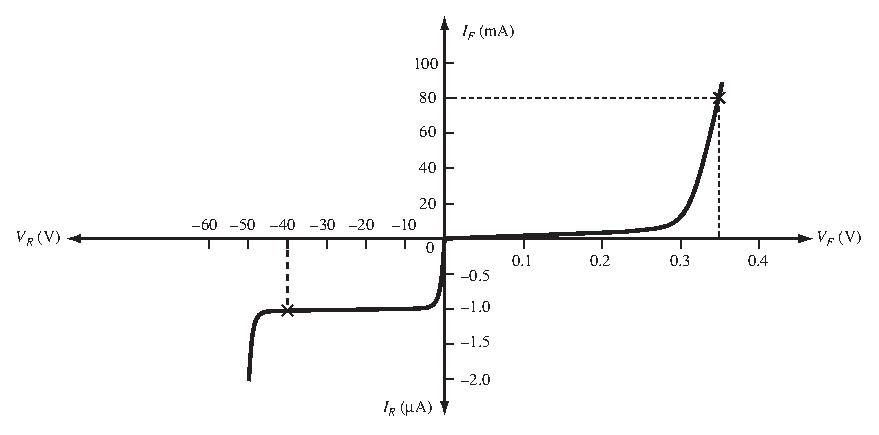
\includegraphics{chap1/S3-EE-01-010.eps}
%\caption{}\label{fig1.7}
\end{figure}
\end{example}

\begin{solution}
Given, $I_F =80 \mA$.

From the characteristics of figure given

at $I_F = 80 \mA$, $V_F = 0.35 V$.

Hence, the static forward resistance is given by 
$$
R_F = \frac{V_F}{I_F} = \frac{0.35 V}{80 \mA} = \frac{0.35 V}{0.08 A} =
4.375 \Omega
$$

From the characteristics

at $V_R = 40 V$, $I_R =1 \mu A$

Hence, the static reverse resistance is given by 
$$
R_R = \frac{V_R}{I_R} = \frac{40 V}{1 \mu A} = 40 M \Omega
$$

Observe that $R_F < < R_R$ as expected. 

Looking at the knee of the characteristics, we can say that the cut in
voltage $V_\gamma$ is approximately 0.3 V.
\end{solution}

\begin{example}\label{exam1.4}
From the characteristics shown below identify the diode and
  give its ratings.
\begin{figure}[H]
\centering
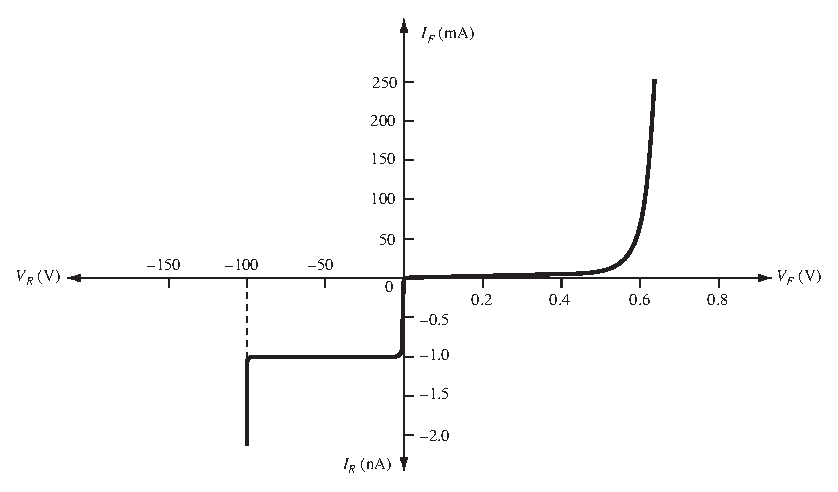
\includegraphics{chap1/S3-EE-01-011.eps}
%\caption{}\label{fig1.7}
\end{figure}
\end{example}

\begin{solution}
Looking at the knee of the characteristics given in Fig, we can say
that the cut-in voltage, 
$$
V_\gamma \sim 0.6 V
$$

Hence, the diode represented in the given characteristics is a Silicon
diode.

{\bf The ratings of the diode are as follows~:}

Maximum forward current, $I_{F(\max)} = 250 \mA$

Cut-in Voltage, $V_\gamma = 0.6 V$

Reverse current, $I_{R\text{(nominal)}} = 1 nA$

Reverse break down voltage, $V_{R\text{(breakdown)}} = 100$~V

Taking a factor of safety of 25\% we can say that 

Maximum reverse voltage, $V_{R(\max)} = 75 V$ 
\end{solution}

\begin{example}\label{exam1.5}
Plot the forward and reverse characteristics of a diode, given the
following data:

Cut-in voltage = 0.6 V

Reverse breakdown voltage = 40 V

Nominal reverse current = 1.0 $\mu$ A

Forward current = 20 mA at a forward voltage of 0.65 V

Forward current = 60 mA at a forward voltage of 0.7 V.
\end{example}

\begin{solution}
Given,

$V_\gamma = 0.6 V$

$V_{R\text{(Breakdown)}} = 40 V$

$I_{R(\text{nominal})} = 1.0\, \mu A$

$I_F = 20 \mA$ at $V_F = 0.65 V$ (point A) and 

$I_F = 60\,mA$ at $V_F = 0.7 V$ (point B).

The forward and reverse characteristics of the diode may be plotted as
shown below.
\begin{figure}[H]
\centering
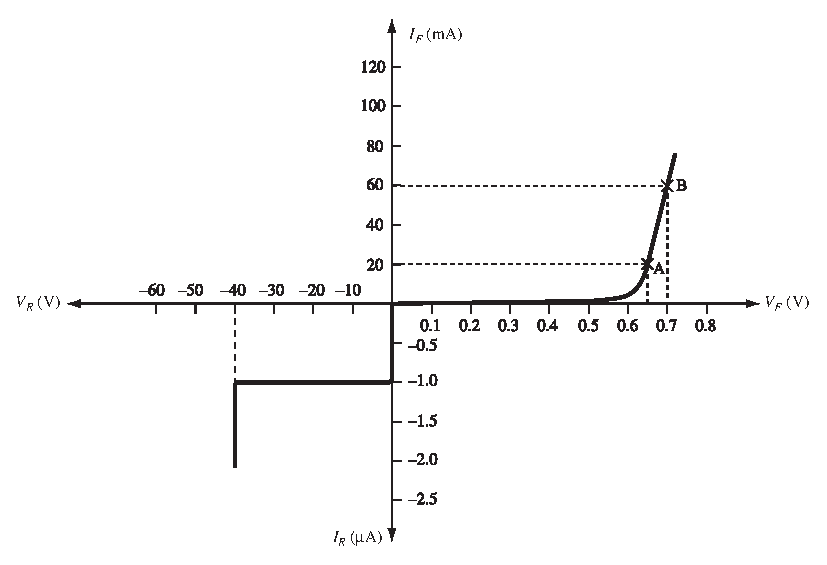
\includegraphics{chap1/S3-EE-01-012.eps}
%\caption{}\label{fig1.7}
\end{figure}
\vskip -1cm
\end{solution}

\eject

\section{Comparison between Silicon and Germanium diodes}\label{sec1.9}
\index{Diode!comparison}

Silicon and Germanium diodes can be compared with reference to
specifications and application as shown in Table 1.1
\begin{table}[H]
\caption{Comparison of Silicon and Germanium diodes}\label{tab1.1}
{\renewcommand{\arraystretch}{1.2}
\begin{tabular}{|l|c|c|c|}
\hline
{\bf Sl.No.} & {\bf Parameter} & {\bf Silicon Diode} & {\bf Germanium Diode}\\
\hline
1. & Material used & Silicon & Germanium\\
\hline
2. & Cut-in Voltage & 0.6\,V & 0.3\,V\\
\hline
3. & Reverse saturation current & Few nA & Few $\mu$\,A\\
\hline
4. & Effect of temperature & Less & More\\
\hline
5. & Break down Voltage & Higher $(> 100\text{\,V})$ & Lower $(<100\text{\,V})$\\
\hline
6. & Applications & 
\begin{tabular}{l@{\;}l}
$\bullet$ & Rectifiers\\[-1pt]
$\bullet$ & Clippers\\[-1pt]
$\bullet$ & Clampers
\end{tabular}
&
\begin{tabular}{l}
Low Voltage\\[-1pt]
low temperature\\[-1pt]
applications
\end{tabular}\\
\hline
\end{tabular}}
\end{table}

\section{Important diode parameters}\label{sec1.10}
\index{Diode!parameters}

Some of the important diode parameters are as follows.
\begin{itemize}
\itemsep=0pt
\item Forward voltage drop, $V_\gamma$
\item Reverse saturation current, $I_{R(\text{nominal})}$ or
  $I_{R \text{(sat)}}$
\item Reverse break down voltage, $V_{BR}$
\item Dynamic resistance, $r_d$
\item Maximum forward current $I_{F (\max)}$
\end{itemize}

The definition of each of these parameters is given below.

\bigskip
\heading{Forward voltage drop:}\index{Forward voltage drop}

\noindent
 It is the voltage drop across a diode when it conducts. The forward
 bias voltage must exceed this voltage before the diode begins to
 conduct large currents. It is also referred to as the cut-in voltage
 $V_\gamma$ and is about 0.6 V to 0.7 V for Silicon diodes and about
 0.2\,V to 0.3 V for Germanium diodes.
 
\heading{Maximum forward current:}\index{Maximum forward current}

\noindent
It is the maximum current a diode can pass under forward bias
condition, without permanent damage to the $p$-$n$ junction due to
over heating. It is denoted as $I_{F(\max)}$. Diode circuits must be
designed for currents well within this value.
 
\medskip
\heading{Reverse saturation current:}\index{Reverse saturation current}

\noindent
The reverse saturation current $I_{R(\text{sat})}$ is the nominal
current, which flows through the diode when it is reverse biased. It
is in the order of $nA$ for Silicon diodes and of the order of $\mu A$
in case of Germanium diodes.

\medskip
\heading{Reverse breakdown voltage:}\index{Reverse breakdown voltage}

\noindent
The reverse breakdown voltage, $V_{BR}$ is the reverse bias voltage at
which the $p$-$n$ junction breaks down and permanently damages the
diode. Diodes which can recover after such breakdown are called Zener
Diodes which have application in voltage regulation. The reverse
breakdown voltage is less than 50 V for Silicon diodes and about 100
V for Germanium diodes.

The dynamic resistance is discussed is the next section.\\[-20pt]

\section{Dynamic resistance of diode and its graphical determination}\label{sec1.11}

The dynamic resistance\index{Diode!dynamic resistance} or $ac$ resistance or incremental resistance,
$r_d$ of a diode is the reciprocal of the slope of the forward
characteristics beyond its knee as illustrated in Fig.~\ref{fig1.8}.
\begin{figure}[H]
\centering
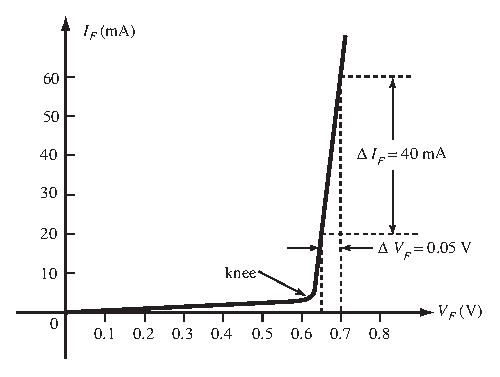
\includegraphics[scale=1.1]{chap1/S3-EE-01-013.eps}
\caption{Forward characteristics showing calculation for $r_{d}$}\label{fig1.8}
\end{figure}

Slope of the forward characteristics $= \dfrac{\Delta I_F}{\Delta
  V_F}$

Dynamic resistance $r_d = $reciprocal of slope of forward
characteristics.
\begin{equation}
\therefore ~ r_d = \frac{\Delta V_F}{\Delta I_F} \label{eq1.3}
\end{equation}

For the characteristics shown in Fig. 1.8.
$$
r_d = \frac{\Delta V_F}{\Delta I_F} = \frac{0.05 V}{40 \mA} =
\frac{0.05 V}{0.04 A} = 1.25 \Omega
$$

This includes the $dc$ resistance of the semiconductor material. The
pure $ac$ resistance can be obtained from the $dc$ forward current by
using the relation
\begin{equation}
r'_d = \frac{0.026}{I_F} \label{eq1.4}
\end{equation}

At, say, an $I_F$ of 40 mA, the pure $ac$ resistance is 
$$
r'_d = \frac{0.026}{40 \mA} = \frac{0.026}{0.04} = 0.65 \Omega
$$

Note that equation 1.4 is valid at $25^\circ$C. 

\begin{example}\label{exam1.6}
Find the dynamic resistance at 40 mA for the diode whose
characteristic is shown below. Also, calculate the pure $ac$ resistance
of the diode at a forward current of 40 mA. Also estimate the value of
the semiconductor substrate resistance.
\begin{figure}[H]
\centering
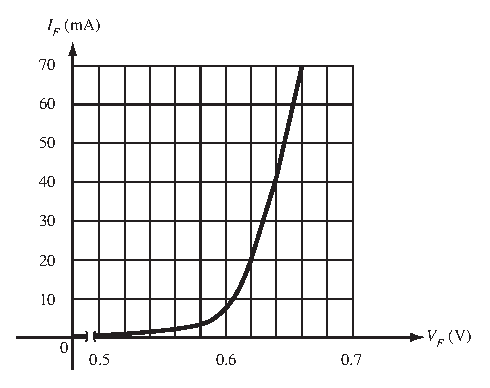
\includegraphics[scale=1.25]{chap1/S3-EE-01-014.eps}
\end{figure}
\end{example}

\begin{solution}
Dynamic resistance, $r_d$ is given by 
$$
r_d = \frac{\Delta V_F}{\Delta I_F}
$$

We are required to find $r_d$ at 40 mA. Let us take two points on the
curve at $(40 \pm 20)$ mA i.e., for $I_F$ = 20 mA and $I_F$ = ~60 mA to
read off $\Delta V_F$ and the corresponding $\Delta I_F$.
\begin{align*}
\text{At~} I_F & = 20 \mA, \qquad V_F = 0.62 ~V\\[3pt]
\text{At~} I_F & = 60 \mA, \qquad V_F = 0.65 ~V\\[3pt]
r_d & = \frac{\Delta V_F}{\Delta I_F} = \frac{(0.65-0.62)V}{(60-20)\mA}
= \frac{0.03V}{40 \mA} = \frac{0.03\text{\,V}}{0.04\text{\,A}} = 0.75 \Omega
\end{align*}

Now the pure $ac$ resistance at 40 mA is given by
$$
r'_d = \frac{0.026}{I_F} = \frac{0.026}{40\mA} = \frac{0.026}{0.04} =
0.65 \Omega
$$

It is easy to see that the semiconductor substrate resistance is 
\begin{align*}
r_{\text{substrate}} & = r_d - r'_d\\
& = 0.75\Omega - 0.65\Omega = 0.1 \Omega
\end{align*}
\vskip -.9cm
\end{solution}

\begin{example}\label{exam1.7}
Find the static forward resistance at a forward current of 20 mA for
the diode whose characteristics is shown below. Further; find the
dynamic resistance at 20 mA using (i) the characteristics and (ii) the
forward current. Estimate the value of the substrate resistance.
\begin{figure}[H]
\centering
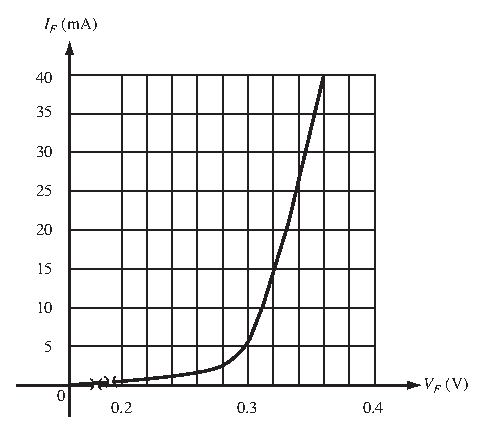
\includegraphics[scale=1.1]{chap1/S3-EE-01-015.eps}
\end{figure}
\end{example}

\begin{solution}
Static forward resistance is given by
$$
R_F = \frac{V_F}{I_F} 
$$

From the characteristics of Fig. given 

at $I_F = 20 \mA$, $V_F = 0.33 V$
$$
R_F = \frac{0.33 V}{20 \mA} = \frac{0.33 V}{0.02 A} = 16.5 \Omega
$$

Dynamic resistance is given by 
$$
r_d = \frac{\Delta V_F}{\Delta I_F}
$$

Let us consider values of $V_F$ for $I_F = (20 \pm 10) \mA$
\begin{align*}
\text{At } ~ I_F & = 10 \mA, \quad V_F = 0.31 V \\
\text{At } ~ I_F & = 30 \mA, \quad V_F = 0.35 V\\
r_d & = \frac{(0.35-0.31)V}{(30-10) \mA} = \frac{0.04 V}{0.02 A} = 2 \Omega
\end{align*}

Dynamic resistance using forward current is given by
\begin{align*}
r'_d & = \frac{0.026}{I_F}\\
\text{At } ~ I_F & = 20~ \mA\\
r'_d & = \frac{0.026}{20 \mA} = \frac{0.026}{0.02} = 1.3 \Omega
\end{align*}

The substrate resistance is given by
$$
r_{\text{substrate}} = r_d - r'_d = 2 \Omega - 1.3 \Omega = 0.7 \Omega.
$$
\vskip -.7cm
\end{solution}

\section{Characteristics of an ideal diode}\label{sec1.12}
\index{Diode!ideal diode}

We have seen that the diode has a very low forward resistance and a
very high reverse resistance. Further, in typical circuit
applications, the $dc$ voltages applied will be in the range of 5 V to
48 V. Thus the knee voltage or forward voltage drop of 0.7 V for
Silicon or 0.3 V for Germanium diode is small when compared to the
circuit voltages.

Ideally, we can say
\begin{itemize}
\item Forward resistance, $R_F = 0$

\item Reverse resistance, $R_R = \infty$

\item Forward voltage drop, $V_\gamma = 0$
\end{itemize}

\vfill\eject

Note that $R_F = 0$ represents a short circuit or a switch in
\textit{closed} condition, while $R_R = \infty$ represents a
\textit{open} circuit or a switch in \textit{open} condition.
$$
R_F = 0 \text{~ implies ~} \frac{\Delta V_F}{\Delta I_F} = 0 \quad
\text{ or } \quad \frac{1}{\Delta V_F / \Delta I_F} = \infty \text{ or
}
$$
slope of the forward characteristics is infinite, represented by a
vertical line. 

$R_R  = \infty$ implies that the slope is zero i.e., a horizontal
line.

$V_\gamma =0$ implies that current rapidly increases for forward
voltage just beyond 0 V.

These characteristics are captured in the ideal characteristics shown
in Fig. 1.9.
\begin{figure}[H]
\centering
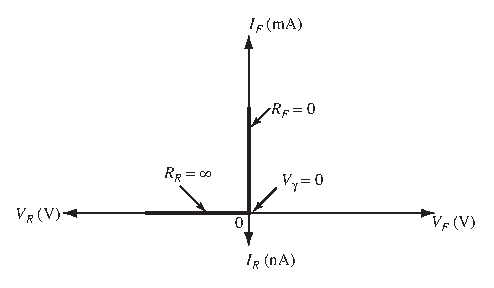
\includegraphics[scale=1.1]{chap1/S3-EE-01-016.eps}
\caption{Ideal diode\index{Ideal diode} characteristics}
\end{figure}

\heading{Approximate characteristics\index{Diode!approximate characteristics} of a Silicon and Germanium diodes}


In most applications, the diode forward voltage drop can be assumed
constant though not zero, since circuit voltages will be much higher
than $V_\gamma$. However, $R_F = 0$ and $R_R = \infty$ is a
near-practical assumption. Hence in most practical cases, the
practical approximation shown in Fig.1.10 may be used for analysis.
\begin{figure}[H]
\centering
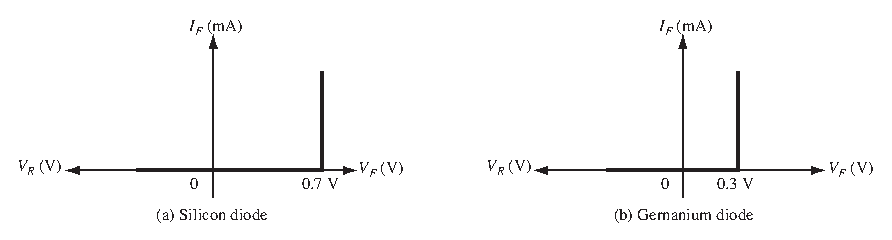
\includegraphics{chap1/S3-EE-01-017.eps}
\caption{Approximate diode characteristics}
\end{figure}

In general we will accept 0.7 V as the forward voltage drop in a
Silicon diode and 0.3 V in a Germanium diode.

\section{Kirchhoff's Voltage Law}\label{sec1.13}

Kirchhoff's voltage law\index{Kirchhoff's voltage law} (KVL) states that the algebraic sum of emfs
and voltage drops in a closed path of a circuit is zero.

Consider the circuit shown in Fig.~\ref{fig1.11}.
\begin{figure}[H]
\centering
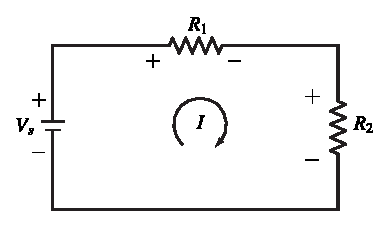
\includegraphics{chap1/S3-EE-01-018.eps}
\caption{Circuit to study the application of KVL}\label{fig1.11}
\end{figure}

The following convention is adopted while writing KVL equation. 

\begin{itemize}
\item[{\rm 1.}] \textbf{Convention for Voltage drop}

Current flows from higher potential point to lower potential
point. Hence potential falls when we go along current and potential
rises when we go against current. There fore
\begin{align*}
\text{along current, } \quad & \text{Voltage drop } = - IR\\
\text{against current,} \quad & \text{Voltage drop } = + IR  
\end{align*}

\item[{\rm 2.}] \textbf{Convention for emfs}

Potential rises when we go from negative terminal to the positive
terminal of the source. Thus emf is taken with positive sign. Emf is
taken with negative  sign when we go from positive to negative
terminal of the source.

Using this convention and writing KVL equation for the circuit of
Fig.~\ref{fig1.11} we have
\begin{align}
V_S - IR_1 - I R_2 & = 0 \notag\\
\text{or } \qquad I (R_1 + R_2) & = V_S  \notag\\
\text{or } \qquad  I & = \frac{V_S}{R_1 + R_2}  \label{eq1.5}
\end{align}

If $V_{S}=12V$, $R_1 = 1 K \Omega$ and $R_2 = 2 K \Omega$ then
\begin{align*}
I &= \frac{V_S}{R_1 + R_2}\\[5pt]
& = \frac{12 V}{(1k \Omega+2k\Omega)}\\[5pt]
& = \frac{12 V}{3
k \Omega} = 4\, m A
\end{align*}
\end{itemize}
 
\begin{example}\label{exam1.8}
Calculate the diode current in the circuit shown assuming a Silicon diode.
\begin{figure}[H]
\centering
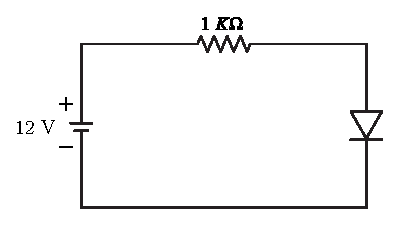
\includegraphics{chap1/S3-EE-01-019.eps}
\end{figure}
\end{example}

\begin{solution}
The circuit with currents and voltages marked is shown below
\begin{figure}[H]
\centering
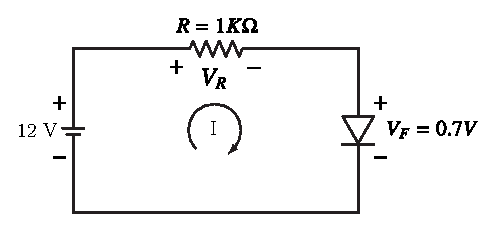
\includegraphics{chap1/S3-EE-01-020.eps}
\end{figure}

Applying Kirchhoff's Voltage Law we have 
\begin{gather*}
12 V - I (1 k \Omega) - 0.7\text{\,V} =0\\[4pt]
I = \frac{12 V - 0.7 V}{1 k \Omega}=11.3\text{\,mA}
\end{gather*}
\vskip -1cm
\end{solution}

\eject


\begin{example}\label{exam1.9}
Repeat Example 1.8 with the single diode replaced by two Silicon
diodes in series. 
\end{example}

\begin{solution}
The circuit with current and voltages marked is shown below.
\begin{figure}[H]
\centering
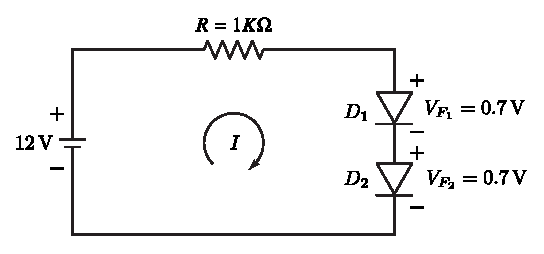
\includegraphics{chap1/S3-EE-01-021.eps}
\end{figure}

Applying Kirchhoff's Voltage Law around the loop,
\begin{align*}
12 V - I (1 k \Omega) - 0.7 V - 0.7 V =0\\[4pt]
\Rightarrow \quad I = \frac{12V - 1.4V}{1 k \Omega} = 10.6 \mA
\end{align*}
\vskip -.9cm
\end{solution}

\smallskip
\begin{example}\label{exam1.10}
Find the forward current in a circuit consisting of a Germanium diode
in series with a 3.3k$\Omega$ resistor and a 9 V battery.
\end{example}

\begin{solution}
The circuit is shown below.
\begin{figure}[H]
\centering
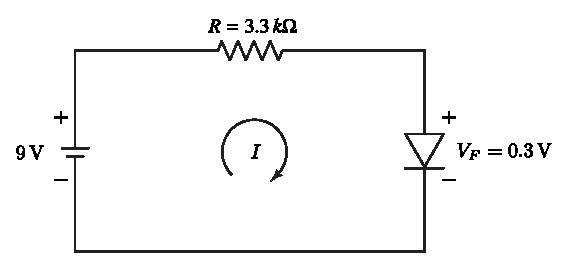
\includegraphics{chap1/S3-EE-01-022.eps}
\end{figure}

The diode drop is 0.3 V for a Germanium diode.

Writing Kirchhoff's Voltage Law around the loop,
\begin{gather*}
9 V - I (3.3 k\Omega) - 0.3 V = 0\\[4pt]
\therefore ~~~ I = \frac{9 V - 0.3 V}{3.3 k \Omega} = 2.64 \mA
\end{gather*}
\vskip -.9cm
\end{solution}

\eject

\begin{example}\label{exam1.11}
A circuit consists of a Silicon diode in series with a $2.7\,k\Omega$ resistor
and a battery. Find the  battery voltage if the forward current is
1.96 mA.
\end{example}

\begin{solution}
The circuit is shown below.
\begin{figure}[H]
\centering
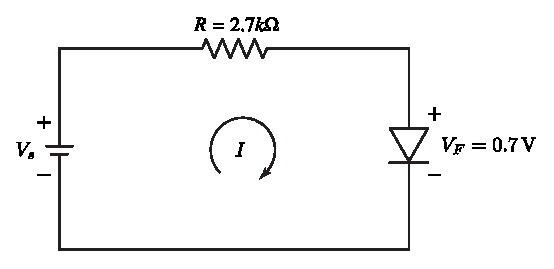
\includegraphics{chap1/S3-EE-01-023.eps}
\end{figure}

Applying Kirchhoff's Voltage Law around the loop,
\begin{align*}
V_S - IR - V_F & = 0\\[3pt]
V_S & = IR + V_F \\[3pt]
& = (1.96 \mA) (2.7 \kk \Omega) + 0.7 \V\\[3pt]
& = 5.992 V \approx 6 \V
\end{align*}

The battery voltage is 6 V.
\end{solution}

\smallskip

\begin{example}\label{exam1.12}
Find the value of the series resistance R, required to drive a
forward current of 1.25 mA through a Germanium diode from a 4.5 V battery.
\end{example}

\begin{solution}
The circuit is shown below.
\begin{figure}[H]
\centering
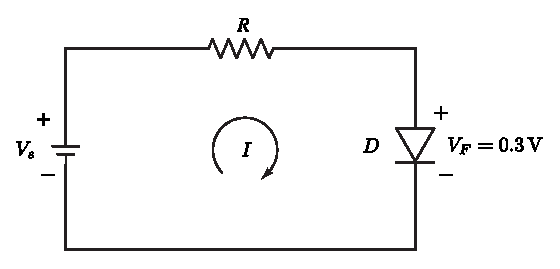
\includegraphics{chap1/S3-EE-01-024.eps}
\end{figure}

\eject

Applying KVL to the circuit shown we have 
\begin{align*}
& V_S - IR  - V_F = 0\\[4pt]
& 4.5 \V - (1.25 \mA) R - 0.3\V =0\\[4pt]
& \Rightarrow ~~ R =\frac{4.5\V - 0.3\V}{1.25 \mA} = 3.36 \kk \Omega.
\end{align*}
\vskip -.9cm
\end{solution}

\section{Piecewise-linear characteristics of diode}\label{sec1.14}
\index{Diode!piecewise-linear characteristics}

The straight line approximation of the forward characteristic of a
diode is called its piecewise linear characteristics. The actual and
the piecewise-linear approximations are shown in Fig.~\ref{fig1.12}.
\begin{figure}[H]
\centering
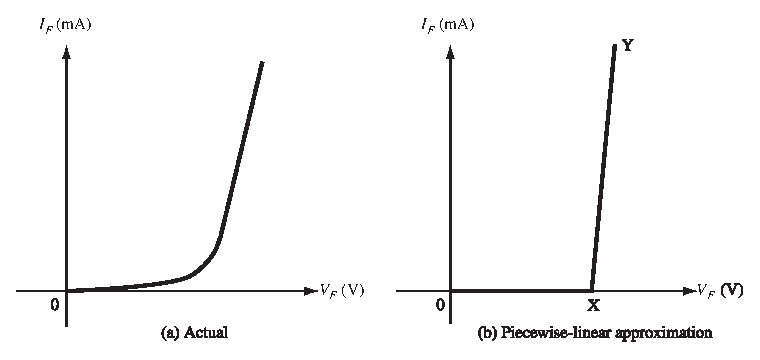
\includegraphics{chap1/S3-EE-01-025.eps}
\medskip
\caption{Typical diode characteristics}\label{fig1.12}
\end{figure}

The piecewise-linear characteristic is constructed by fixing the
forward diode voltage drop at point $X$ and then drawing a segment
$XY$ with a slope given by the reciprocal of the dynamic resistance of
the diode.

For Silicon diode, voltage at point $X$ is 0.7 V.

For Germanium diode, voltage at point $X$ is 0.3 V.


\begin{example}\label{exam1.13}
Plot the piecewise-linear characteristic of a Silicon diode with a
dynamic resistance of 0.2 $\Omega$ and a maximum forward current of
200 mA.
\end{example}

\begin{solution}
A Silicon diode has a forward voltage drop of 0.7V.

Draw the voltage and current axis and mark point $X$ at 0.7 V on the
$V_F$ axis as shown in the figure given below.
\begin{figure}[H]
\centering
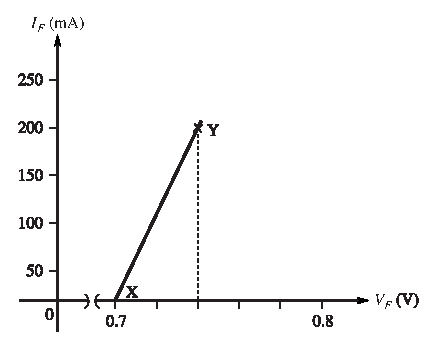
\includegraphics{chap1/S3-EE-01-026.eps}
\end{figure}

By definition, 
$$
r_d = \frac{\Delta V_F}{\Delta I_F}
$$

For a $\Delta I_F$ of 200 mA,
$$
\Delta V_F = r_d \times \Delta I_F = 0.2\Omega \times 0.2A = 0.04 \V
$$

Now mark the point $Y$ at $I_F = 200\mA$ and 
$$
V_F = V + \Delta V_F = 0.7V + 0.04V = 0.74 \V
$$

Join $XY$ to get the piecewise-linear approximation of the diode
characteristic.
\end{solution}

\begin{example}\label{exam1.14}
Obtain the piecewise-linear characteristic of a Germanium diode with a
dynamic resistance of 0.5 $\Omega$ and a maximum forward current of
100 mA.
\end{example}

\begin{solution}
Draw the voltage and current axis and mark the point $X$ on the
voltage axis at 0.3 V (Germanium diode) as shown in the figure.
\begin{figure}[H]
\centering
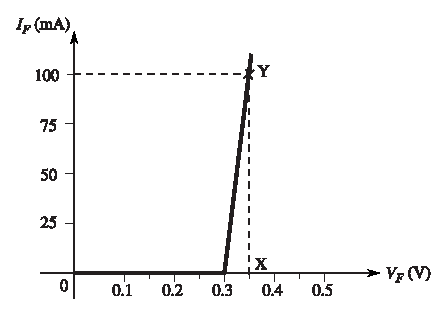
\includegraphics{chap1/S3-EE-01-027.eps}
\end{figure}

Now,
\begin{align*}
r_d & = \frac{\Delta V_F}{\Delta I_F}\\[3pt]
\text{For } \quad \Delta I_F & = 100 \mA,\\[3pt]
\Delta V_F & = r_d \times I_F = 0.5\Omega \times 0.1A = 0.05 \V
\end{align*}

Mark the point $Y$ at $I_F = 100\mA$ and $V_F = V + \Delta V_F = 0.3V +
0.05V = 0.35 \V$. Join $XY$ to get the piecewise-linear characteristic.
\end{solution}

\section[$dc$ equivalent circuit of diode]{\boldmath$dc$ equivalent circuit of diode}\label{sec1.15}
\index{Diode!equivalent circuit}

The equivalent circuit of a diode is a model which closely approximates the actual behaviour of the diode under specific operating conditions. It is useful in the analysis of circuits containing diodes. In its simplest form the equivalent circuit of a diode contains a voltage source and a resistance.

From the piecewise linear characteristic of Fig.~\ref{fig1.12}(b) we observe the following facts.
\begin{itemize}
\item[$\bullet$] For $V_{F}<V_{\gamma}$, the diode current is zero. Hence a voltage source of value $V_{\gamma}$ is placed in the forward current path, with a polarity to oppose the forward current flow for $V_{F}<V_{\gamma}$.

\item[$\bullet$] For $V_{F}\geq V_{\gamma}$, the diode current increases linearly with the diode voltage. Since $r_{d}=\dfrac{\Delta V_{F}}{\Delta I_{F}}$ or $\Delta V_{F}=r_{d}\Delta I_{F}$, a resistance $r_{d}$ is placed in series with the voltage source.
\end{itemize}

The piecewise linear equivalent circuit of a diode is shown in Fig.~\ref{fig1.13}(b).

If $r_{d}=0$, the equivalent circuit contains only the voltage source as shown in Fig.~\ref{fig1.13}(c).
\begin{figure}[H]
\centering
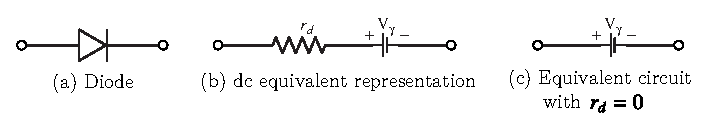
\includegraphics[scale=1.1]{chap1/S3-EE-01-029.eps}
\caption{Diode and its equivalent circuit using piecewise-linear model}\label{fig1.13}
\end{figure}

\eject

\begin{example}\label{exam1.15}
Obtain the values of the diode current for the circuit shown below
with 

(a)~ $r_d =0$ (b)~ $r_d = 0.2 \Omega$
\begin{figure}[H]
\centering
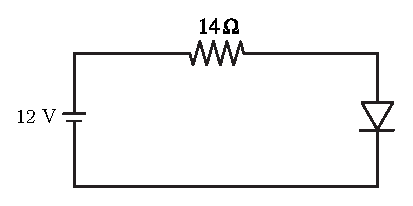
\includegraphics{chap1/S3-EE-01-UN001.eps}
\end{figure}
\end{example}

\begin{solution}
\begin{itemize}
\item[(a)] With $r_d = 0$, let us replace the diode by its equivalent
  circuit shown in Fig.\ref{fig1.13}(c) assuming a Silicon diode.
\begin{figure}[H]
\centering
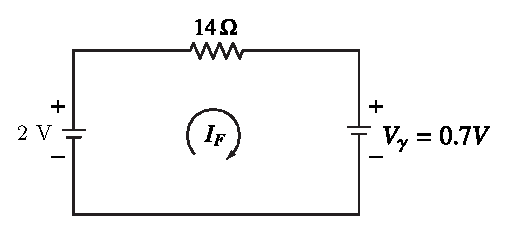
\includegraphics{chap1/S3-EE-01-030.eps}
\end{figure}

Applying Kirchhoff's Voltage Law,
\begin{align*}
2 \V - I_F\, (14\Omega) - 0.7 \V  & = 0\\[4pt]
\Rightarrow \quad I_F = \frac{2V - 0.7 V}{14\, \Omega} & = 0.1 A\\[4pt]
\text{or}\qquad I_F & = 100 \mA
\end{align*}

\item[(b)] With $r_d = 0.2\Omega$ the equivalent circuit is shown
  below
\begin{figure}[H]
\centering
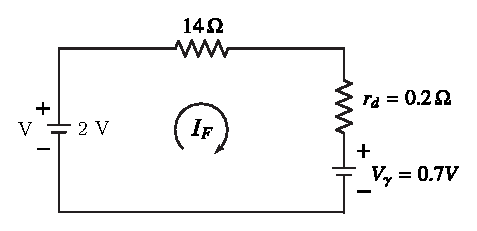
\includegraphics{chap1/S3-EE-01-031.eps}
\end{figure}

\eject

Applying Kirchhoff's Voltage Law,
\begin{align*}
2 \V - I_F \,(14 \Omega) - I_F\, (0.2 \Omega) - 0.7 \V & = 0\\[3pt]
\Rightarrow ~~ I_F & = \frac{2\V - 0.7 \V}{14 \Omega + 0.2 \Omega}\\[3pt]
& = 98.6 \mA
\end{align*}
\end{itemize}
\vskip -.9cm
\end{solution}

\begin{example}\label{exam1.16}
Find the value of resistor R in the circuit shown below using
Germanium diode with a dynamic resistance of $0.5 \Omega$ for a
circuit current of 174 mA.
\begin{figure}[H]
\centering
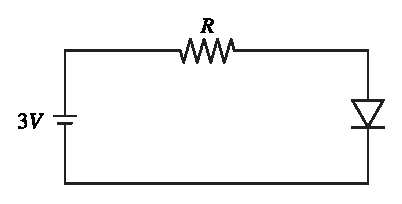
\includegraphics{chap1/exp1.16.eps}
\end{figure}
\end{example}

\begin{solution}
The equivalent circuit is shown below.
\begin{figure}[H]
\centering
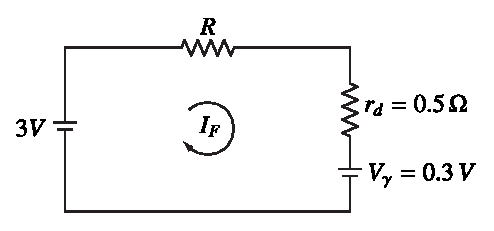
\includegraphics[scale=.95]{chap1/sol1.16.eps}
\end{figure}

Given, $r_d = 0.5 \Omega$, $I_F = 174 \mA$, $V_\gamma =0.3 \V$
(Germanium diode). 

\smallskip

Writing Kirchhoff's Voltage Law equation,
\begin{align*}
3 \V - (1.74 \mA) & R - (1.74 \mA) (0.5 \Omega) - 0.3 \V = 0\\[4pt]
\Rightarrow ~~ R & = \frac{3\V - (1.74 \mA) (0.5\Omega)-0.3 \V}{1.74
  \mA}\\[4pt]
& = 15.01 \Omega
\end{align*} 

Choose $R = 15 \Omega$
\end{solution}

\eject

\section{DC load line}\label{1.16}

A DC load line\index{Diode!dc load line} is a straight line on the diode forward characteristic
which describes all the $dc$ conditions that exist in the operation of
the circuit.

Consider a diode series circuit as shown in Fig.~\ref{fig1.14}.
\begin{figure}[H]
\centering
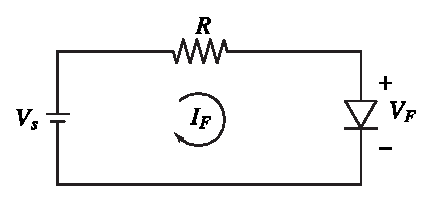
\includegraphics{chap1/fig1.14.eps}
\caption{Diode Series Circuit}\label{fig1.14}
\end{figure}
where 

\vskip .1cm
~~~ $I_F = $ Current through the diode

~~~ $V_F =$ Voltage across the diode
\vskip .1cm

The following values are chosen for circuit parameters.
$$
V_{S}=4\,V\quad R=100\Omega\quad V_{F}=0.7\,V~\text{(Silicon diode)}
$$

The DC load line is drawn on the diode forward characteristic.
\begin{figure}[H]
\centering
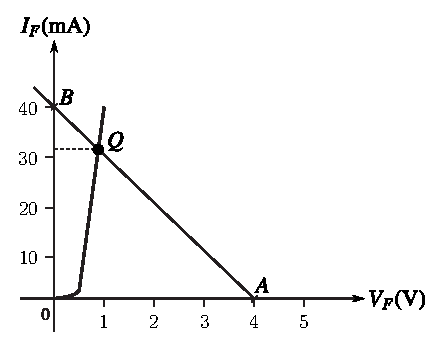
\includegraphics{chap1/fig1.15.eps}
\caption{Plot of DC load line}\label{fig1.15}
\end{figure}

\eject

The load line is plotted with any two values of circuit
current-voltage pair. Applying Kirchhoff's Voltage Law to the circuit
in Fig.~\ref{fig1.14}.
\begin{gather}
V_S - I_F R - V_F = 0 \notag\\
V_S = I_F R + V_F \label{eq1.6}
\end{gather}
is the equation of the load line.

\vskip .1cm
From Eqn.~\ref{eq1.6}.

\vskip .1cm
For $I_F = 0$, $V_F = V_S$

\vskip .1cm
$\therefore~~ V_F = V_S$, $I_F = 0$ is one point on the load line,
marked as A in Fig.~\ref{fig1.15} at
$$
V_F = 4 \V, ~~ I_F = 0 \mA
$$

Again from equation 1.6

\vskip .1cm
For $V_F = 0$, $I_F = \dfrac{V_S}{R}$

\vskip .1cm
$\therefore$~ $V_F = 0$, $I_F = \dfrac{V_S}{R}$ is a second point on
the load line, marked as B in Fig.~\ref{fig1.15} at 
$$
V_F = 0, ~ I_F = \frac{4 V}{100\, \Omega} = 40 \mA
$$

Join AB to get the DC load line. Observe that the DC load line
intersects the diode characteristic at the point $Q$ which corresponds
to $I_F = 33 \mA$ and $V_F = 0.7 \V$ as expected. This can be verified
from equation (1.6)
\begin{align*}
I_F & = \frac{V_S - V_F}{R}\\[3pt]
V_F & = 0.7 \V \text{ ~ for Silicon diode}\\[3pt]
\therefore ~~ I_F & = \frac{4\V - 0.7 \V}{100 \Omega} = 33 \mA
\end{align*}

\section{Need for graphical analysis or DC load line}\label{sec1.17}

The diode forward current in a circuit can be determined approximately
by using Kirchhoff's Voltage Law, assuming that the diode voltage drop
is constant. We have been taking it as 0.7 V for Silicon diode and
0.3 V for Germanium diode. However, in reality this is not the case
since the characteristic is not a vertical line. The exact value of
the forward current through the diode and voltage drop across the
diode can be found at the intersection of the DC load line and the
diode forward characteristic.

\section{Meaning of Q-point}\label{sec1.18}

The intersection of the diode forward characteristic and the DC load
line is called the $Q$-point,\index{Q@$Q$-point} also referred to as the quiescent point
or the $dc$ bias point. The equation of the load line as given by
equation 1.6 is
$$
V_S = I_F R + V_F
$$

It is easy to see that for a given battery voltage $V_S$ and for a
fixed external resistor $R$, the value of $I_F$ and $V_F$ as defined
by the $Q$-point\index{Diode!Q@$Q$-point} is the only possible value. This external resistor
is usually called the load resistor and denoted as $R_L$.

\begin{example}\label{exam1.17}
Find the load resistance in the circuit shown using the diode forward
characteristic provided.
\begin{figure}[H]
\centering
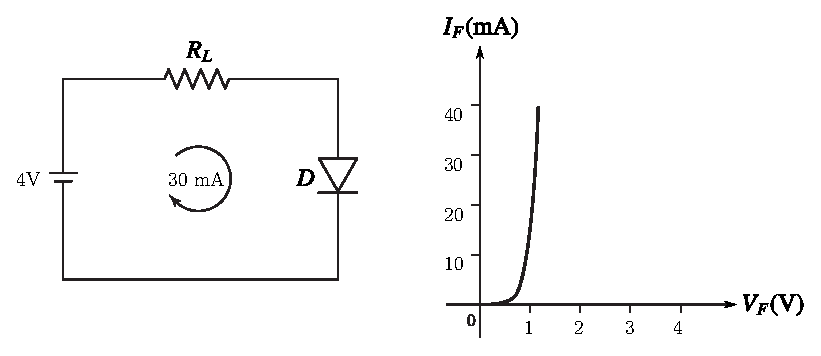
\includegraphics[scale=.8]{chap1/exp1.17.eps}
\end{figure}
\end{example}

\begin{solution}
Applying KVL to the given circuit, 
\begin{equation*}
V_S = I_F R_L + V_F \tag{A}
\end{equation*}

For $I_F = 0 \mA$, $V_F = V_S$

$\therefore$ Mark point $A$ at $I_F = 0$, $V_F = V_S = 4 \V$ as shown
in the Figure
\begin{figure}[H]
\centering
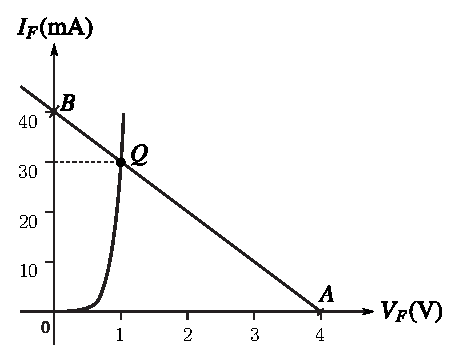
\includegraphics[scale=.8]{chap1/sol1.17.eps}
\end{figure}

Next mark the point $Q$ on the diode characteristic that corresponds
to $I_F = 30$ mA 

Join AQ to meet the $I_F$ axis at $B$.

Putting $V_F = 0$ in equation (A),
$$
R_L = \frac{V_S}{I_F}
$$

But $I_F = 40$ mA at $V_F = 0$
$$
\therefore ~~ R_L = \frac{4V}{40 \mA} = 100\,\Omega
$$
\vskip -.8cm
\end{solution}

\medskip
\begin{example}\label{exam1.18}
A diode with its forward characteristic as shown below is connected in
series with a resistance of $100\,\Omega$ and is driven by a $dc$
voltage source. Calculate the value of the $dc$ supply voltage for a
circuit current of $50\mA$ . Draw the DC load line.
\begin{figure}[H]
\centering
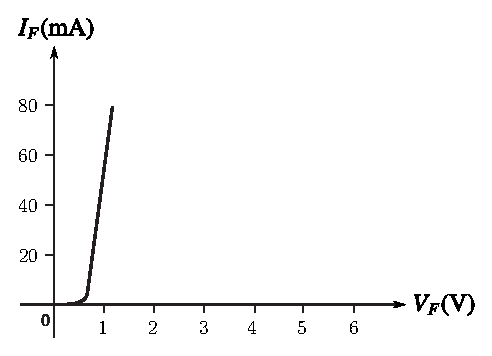
\includegraphics[scale=.85]{chap1/exp1.18.eps}
\end{figure}
\end{example}

\begin{solution}
Fix the point $Q$ on the characteristic at $I_F = 50\mA$ as shown in
the figure given below

Corresponding to this point $V_F = 1\V$.

KVL equation for the circuit is 
\begin{align*}
V_S & = I_F R_L + V_F \\[3pt]
& = (50 \mA) (100\Omega) + 1 \V\\[3pt]
& = 6 \V 
\end{align*}

Mark the point $V_F = 6 \V$ for $I_F = 0\mA$ as B on the $V_F$
axis. Join $BQ$ to draw the $DC$ load line.
\begin{figure}[H]
\centering
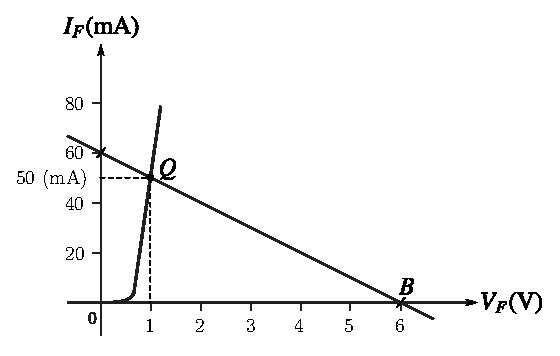
\includegraphics[scale=.9]{chap1/sol1.18.eps}
\end{figure}


\section{Capacitive effects in $p$-$n$ junction}\label{sec1.19}

The capacitive effects\index{Diode!capacitive effects} in a $p$-$n$ junction are
\begin{itemize}
\item[$\bullet$] the depletion layer capacitance or transition capacitance
  which occurs at the junction of a reverse-biased diode.

\item[$\bullet$] the diffusion capacitance which occurs at the junction of
  a forward-biased diode.
\end{itemize}
\vskip -.8cm
\end{solution}

\subsection{Depletion layer capacitance}\label{subsec1.19.1}
\index{Depletion layer capacitance}

When a diode is reverse biased the depletion region around the
junction behaves like a dielectric as this region is free of
carriers. Further, the width of the depletion region increases with
increase in reverse-bias voltage. We know that a dielectric between
two conducting plates acts a capacitor given by,
\begin{equation}
C = \frac{\epsilon\, A}{d} \label{eq1.7}
\end{equation}

Where

\smallskip
C = capacitance in Farads

\vskip .1cm
A = area of the plates in $m^2$

\vskip .1cm
$d$ = distance between the plates in $m$ (which is the width of the
depletion layer) and 

\vskip .1cm
$\epsilon$ = permittivity of the dielectric between the plates in
Farads/m.

\medskip

The depletion layer capacitance,\index{Diode!depletion layer capacitance} $C_{pn}$ can be calculated using the
equation of a parallel-plate capacitor as given in Eqn.~\eqref{eq1.7}.

\eject

Hence the depletion layer capacitance or transition capacitance is the
capacitance of a reverse biased $p$-$n$ junction represented
symbolically as shown in Fig.~\ref{fig1.16}.

The depletion layer capacitance of a low-current diode is typically 4 pF.
\begin{figure}[H]
\centering
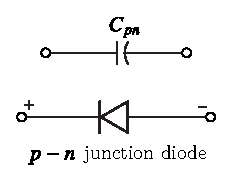
\includegraphics{chap1/fig1.16.eps}
\caption{Representation of depletion layer capacitance}\label{fig1.16}
\end{figure}

\subsection{Diffusion capacitance}\label{subsec1.19.2}
\index{Diode!diffusion capacitance}

When the voltage applied to a forward-biased $p$-$n$ junction is
suddenly reversed, a large reverse current initially flows, which
decreases gradually to the reverse saturation value of the
current. The reverse saturation current is a small current, which flows
when a $p$-$n$ junction is reverse biased as we see in the diode
characteristics. The effect is similar to that of the discharge of a
capacitor and is represented by a capacitance called diffusion
capacitance,\index{Diffusion capacitance} $C_d$ as shown in Fig.~\ref{fig1.17}.
\begin{figure}[H]
\centering
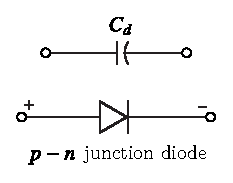
\includegraphics{chap1/fig1.17.eps}
\caption{Representation of diffusion capacitance}\label{fig1.17}
\end{figure}

Thus, diffusion capacitance is defined as the incremental capacitance
given by the rate of change of injected charge with voltage.
\begin{equation}
\text{i.e., } \quad C_d = \frac{dQ}{dV} \label{eq1.8}
\end{equation}
where $Q$ is injected charge and $V$ is the forward-bias
voltage. Generally, it is in the order of\break 1 nF for low current diodes.

\eject

\section[$ac$ equivalent circuit of a diode, under reverse and forward
biased conditions]{\boldmath$ac$ equivalent circuit of a diode, under reverse and forward
biased conditions}\label{sec1.20}
\index{Diode!ac equivalent circuit}


\begin{itemize}
\item {\bf Reverse-biased condition~:}

The equivalent circuit of a reverse -biased diode is shown in
Fig.~\ref{fig1.18}.

It consists of the large reverse resistance $R_R$ in parallel with
depletion layer capacitance $C_{pn}$.
\begin{figure}[H]
\centering
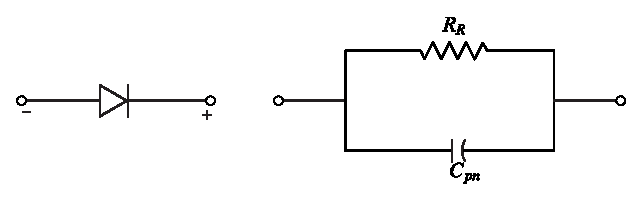
\includegraphics{chap1/fig1.18.eps}
\caption{Reverse-biased diode and its equivalent circuit}\label{fig1.18}
\end{figure}

\item {\bf Forward-biased condition~:}

The equivalent circuit of a forward-biased diode is shown in
Fig.~\ref{fig1.19}. A forward-biased diode is represented by two parallel
circuits as shown in Fig.~\ref{fig1.19}. The first circuit comprises of forward
voltage drop $V_\gamma$ in series with dynamic resistance $r_d$, while
the second circuit contains the diffusion capacitance $C_d$.
\begin{figure}[H]
\centering
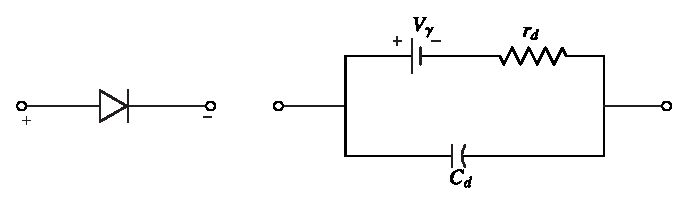
\includegraphics{chap1/fig1.19.eps}
\caption{Forward-biased diode and its equivalent circuit}\label{fig1.19}
\end{figure}

The $ac$ equivalent circuit can be obtained by shorting the $dc$
sources of Fig.~\ref{fig1.19} and is as shown in Fig.~\ref{fig1.20}.
\begin{figure}[H]
\centering
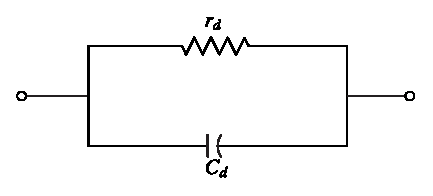
\includegraphics{chap1/fig1.20.eps}
\caption{$ac$ equivalent circuit of a forward-biased junction}\label{fig1.20}
\end{figure}
\end{itemize}

\section{Reverse-recovery time in a diode}\label{sec1.21}
\index{Diode!reverse-recovery time}

When a forward-biased diode is suddenly reverse biased, the time
required for the current to decrease to its reverse saturation value
is called the reverse-recovery time\index{Reverse-recovery time} denoted by $t_{rr}$.

Consider a voltage pulse with a positive and negative voltage, applied
to a diode. The diode current in response to the pulse is shown in
Fig.~\ref{fig1.21}.
\begin{figure}[H]
\centering
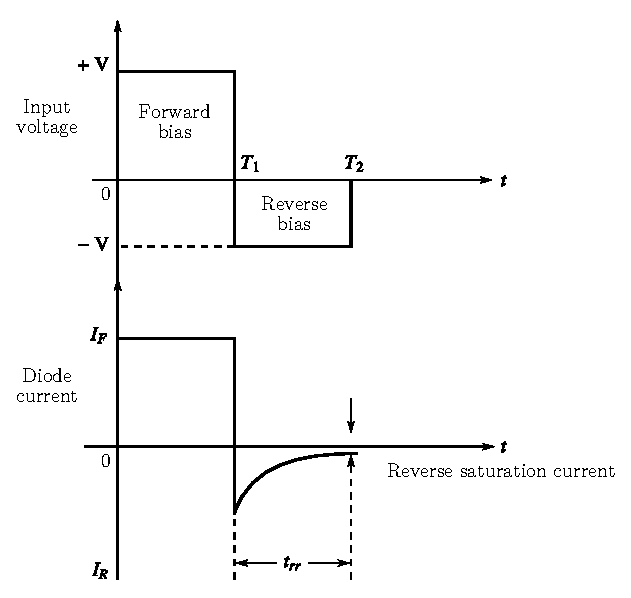
\includegraphics[scale=.91]{chap1/fig1.21.eps}
\caption{Reverse-recovery in a diode}\label{fig1.21}
\end{figure}

When the diode is forward biased, it conducts a forward current
$I_F$. When the pulse instantly switches to a negative value at $t =
T_1$, the diode does not instantly switch off, but conducts current
$I_R = I_F$ initially in the reverse direction. This current gradually
decreases to zero as shown in Fig.~\ref{fig1.21}.

\section{Junction Breakdown in diodes}\label{sec1.22}
\index{Breakdown}

When a Junction diode is reverse biased, only a very small reverse saturation current, $I_{S}$ flows through the Junction. When the reverse voltage is sufficiently high, the junction breaks down and a large reverse current flows. This large reverse current may destroy the diode due to excessive power dissipation. The reverse current and hence the power dissipation can be kept at a safe level by connecting a resistor $R_{1}$ in series with the diode as shown in Fig.~\ref{fig1.25}(a). Fig.~\ref{fig1.25}(b) shows the reverse characteristics of the diode.
\begin{figure}[H]
\centering
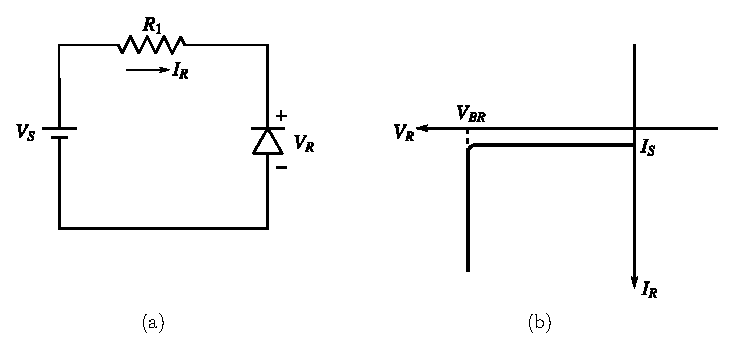
\includegraphics{chap1/fig1.25.eps}
\caption{(a) current limiting for safe operation under reverse break down\\\qquad\quad (b) reverse characteristics of diode}\label{fig1.25}
\end{figure}

Under this condition, the diode may be operated continuously in reverse breakdown. The reverse current returns to its normal level when the reverse voltage is reduced below the reverse breakdown level.

There are two mechanisms that cause breakdown\index{Diode!breakdown} in a reverse biased $pn$ junction.
\begin{itemize}
\item Avalanche Breakdown.

\item Zener Breakdown.
\end{itemize}


\subsection{Avalanche Breakdown}\label{sec1.22.1}
\index{Avalanche Breakdown}

As the reverse voltage across the diode increases, the velocity of minority carriers responsible for the reverse saturation current $I_{S}$ will also increase. Eventually the velocity and the associated kinetic energy of these minority carriers will be sufficiently large to release additional carriers, through collisions with atomic structure. This results in an ionisation process due to which the valence electrons absorb sufficient energy to leave the parent atom. These additional carriers can then aid the ionisation process to the point where a high avalanche current is established and the diode operates in the avalanche breakdown region. Avalanche breakdown occurs in diodes having wide depletion region and is normally produced by reverse voltage levels above 5V.\\[-22pt]

\subsection{Zener Breakdown}\label{sec1.22.2}
\index{Zener Breakdown}

The reverse voltage required for  Avalanche breakdown can be greatly reduced to a value less than 5V, by increasing the doping levels in the $p$ and $n$ type materials. The reduction in depletion region gives rise to a strong electric field in the region of the junction. This strong electric field can disrupt the bonding forces with in the atom and generate the carriers. This mechanism is called zener breakdown and it results in a sharp change in the characteristic. This sharp change in characteristics at low levels of reverse voltage is called the zener region and the voltage at which the zener breakdown occurs is called the zener breakdown voltage, $V_{Z}$ as indicated in Fig.~\ref{fig1.26}.
\begin{figure}[H]
\centering
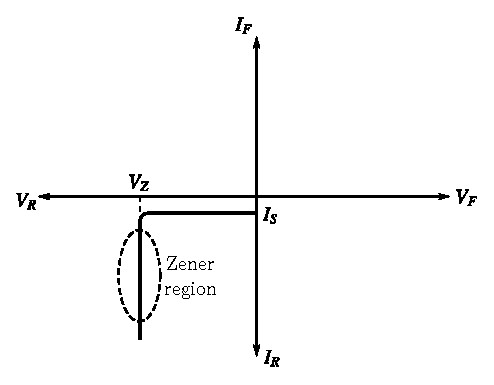
\includegraphics[scale=.9]{chap1/fig1.26.eps}
\caption{Zener region}\label{fig1.26}
\end{figure}

The diodes employing the zener region of the characteristic of a $p$-$n$ junction are called zener divides. Diodes designed for operation in reverse breakdown are found to have a breakdown voltage that remains extremely stable over a wide range of current levels. By virtue of this property the breakdown diodes find application as voltage reference sources. Although zener and avalanche are two different types of breakdown, the name zener diode is commonly applied to all breakdown diodes.\index{Breakdown diodes}\\[-22pt]

\section[Zener Diode and Its $V$-$I$ Characteristics]{Zener Diode and Its \boldmath$V$-$I$ Characteristics}\label{sec1.23}

Zener diode\index{Zener diode} is a breakdown diode with a very narrow depletion region, specially designed to breakdown at small reverse voltages $(<5\text{V})$. When the applied reverse voltage exceeds the breakdown voltage, $V_{Z}$, the reverse current in the diode increases sharply with the voltage across the diode remaining constant at $V_{Z}$. By varying the doping level, the location of zener region can be controlled. With an increase in doping, the number of added impurities increases resulting in the decrease in the zener breakdown voltage $V_{Z}$. Zener diodes are available having zener voltages of 1.8 to 200V with power ratings from 0.25 to 50W.

Fig.~\ref{fig1.27} shows the circuit symbol of zener diode. Note that the symbol is same as that of an ordinary diode but with the cathode bar approximately in the shape of a letter $Z$.
\begin{figure}[H]
\centering
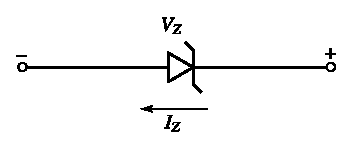
\includegraphics[scale=.9]{chap1/fig1.27.eps}
\caption{Circuit symbol of Zener diode}\label{fig1.27}
\end{figure}

For operation in reverse bias, the voltage drop, $V_{Z}$, is positive on cathode and negative on anode.
\begin{figure}[H]
\centering
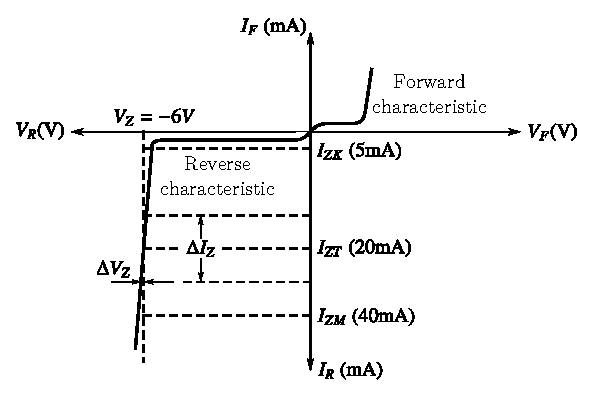
\includegraphics[scale=.95]{chap1/addfig1.28.eps}
\caption{Characteristics of Zener diode}\label{fig1.28}
\end{figure}

Fig.~\ref{fig1.28} shows the typical characteristics\index{Zener diode!characteristics} of a zener diode. Observe that, the forward characteristic is same as that of an ordinary forward biased $p$-$n$ junction doide. The values of $V_{Z}$, $I_{ZT}$ and $I_{ZM}$ indicated on the characteristics are the typical values of the diode under consideration.

\section{Zener diode parameters}\label{sec1.24}

Following are the important parameters\index{Zener diode!parameters} of a zener diode, which are also indicated on the reverse characteristic of Fig.~\ref{fig1.28}. The definition of each of these parameters is given below.

\medskip
\heading{1.~ Zener Breakdown Voltage, \boldmath$V_{Z}$}

\smallskip
It is the reverse-bias voltage at which the zener diode enters the break down region, maintaining a constant voltage $V_{Z}$ across the diode.

\medskip
\heading{2.~ Minimum Reverse Current, \boldmath$I_{ZK}$}

\smallskip
It is the reverse current at the knee of the reverse characteristic and is the minimum reverse current to sustain the breakdown condition.

\medskip
\heading{3.~ Test Current, \boldmath$I_{ZT}$}

\smallskip
It is the current that must be passed through the zener diode while measuring the breakdown voltage $V_{Z}$.

\medskip
\heading{4.~ Maximum Zener Current, \boldmath$I_{ZM}$}

\smallskip
It is the maximum current the diode can carry without exceeding the maximum power dissipation ($P_{D}$).

\medskip
\heading{5.~ Maximum Power Dissipation, \boldmath$P_{D}$}

\smallskip
It is the maximum power which the zener diode can dissipate without destruction. It is given by the product of $V_{Z}$ and $I_{ZM}$.
\begin{equation}
\text{i.e.,}\qquad P_{D}=V_{Z}\,I_{ZM}
\end{equation}

\medskip
\heading{6.~ Dynamic Impedance, $Z_{Z}$}

\smallskip
It defines how $V_{Z}$ charges with variations in diode reverse current. It is defined by
\begin{equation}
Z_{Z}=\dfrac{\Delta V_{Z}}{\Delta I_{Z}}
\end{equation}

\eject

\begin{example}\label{exam1.19}
The circuit shown, uses a Zener with $V_{Z}=7.5V$. Find the diode current and the power dissipation.
\begin{figure}[H]
\centering
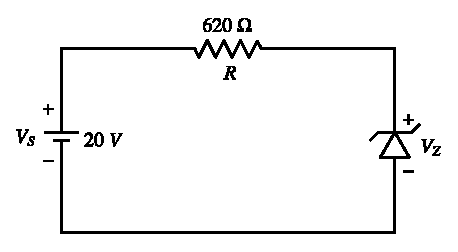
\includegraphics{chap1/exp1.19.eps}
\end{figure}
\end{example}

\begin{solution}
The circuit with currents and voltages marked is shown below.
\begin{figure}[H]
\centering
\includegraphics{chap1/sol1.19.eps}
\end{figure}

Since, $V_{S}>V_{Z}$, the Zener diode operates in breakdown region.

Applying Kirchhoff's Voltage Law around the loop,
\begin{align*}
&V_{S}-I_{Z}R-V_{Z}=0\\[3pt]
&20V-I_{Z}\,(620\Omega)-7.5V=0\\[3pt]
\Rightarrow\qquad & I_{Z}=\dfrac{20V-7.5V}{620\Omega}\\[3pt]
\therefore\qquad & I_{Z}=20.16\text{\;mA}
\end{align*}

Power dissipation in the Zener is given by
\begin{align*}
P_{D} &= V_{Z}I_{Z}=7.5\text{\,V}\times 20.16\text{\;mA}\\[3pt]
&= 151.2\text{\;mW}
\end{align*}
\vskip -.95cm
\end{solution}

\eject

\begin{example}\label{exam1.20}
A 4.3V Zener diode is connected in series with a 820\,$\Omega$ resistor and a $dc$ supply of 12\,V. Find the diode current and the power dissipation.
\end{example}

\begin{solution}
The circuit is shown below.

Since, $V_{S}>V_{Z}$, the Zener diode operates in breakdown region.
\begin{figure}[H]
\centering
\includegraphics{chap1/sol1.20.eps}
\end{figure}

By writing Kirchhoff's Voltage Law equation around the loop,
\begin{align*}
& V_{S}-I_{Z}R-V_{Z}=0\\[4pt]
& I_{Z} = \dfrac{V_{S}-V_{Z}}{R}\\[4pt]
&\quad\! =\dfrac{12V-4.3V}{820\,\Omega}\\[4pt]
&\quad\! = 9.4\text{\,mA}
\end{align*}
and
$$
P_{D}=V_{Z}\,I_{Z}=4.3\text{\,V}\times 9.4\text{\,mA}=40.42\text{\,mW}
$$
\vskip -.85cm
\end{solution}

\section{Equivalent Circuit of Zener Diode}\label{sec1.25}

We know that the Zener diode is operated in the reverse-biased mode to use the constant voltage property beyond breakdown. The $dc$ equivalent circuit of a Zener diode is shown in Fig.~\ref{fig1.29}.

It consists of a voltage source with a voltage of $V_{Z}$ volts. This equivalent circuit\index{Zener diode!equivalent circuit} is used for all $dc$ analysis.
\begin{figure}[H]
\centering
\includegraphics{chap1/fig1.29.eps}
\caption{$dc$ equivalent circuit of Zener diode}\label{fig1.29}
\end{figure}

The $ac$ equivalent circuit is shown in Fig.~\ref{fig1.30}.

It consists of a voltage source with value $V_{Z}$ volts in series with an impedance $Z_{Z}$. The $ac$ equivalent circuit is used in analysis where the Zener current varies by small amounts.

The equivalent circuits given in Fig.~\ref{fig1.29} and Fig.~\ref{fig1.30} are valid only when the diode is operated in the reverse breakdown region.
\begin{figure}[H]
\centering
\includegraphics{chap1/fig1.30.eps}
\caption{$ac$ equivalent circuit of Zener diode}\label{fig1.30}
\end{figure}

\section{Applications of Zener Diode}
Some of the important applications\index{Zener diode!applications} of Zener diode are listed below.
\begin{itemize}
\item It is used as voltage regulator in $dc$ power supplies.

\item Since it limits the voltage under reverse bias, it is used to protect measuring instruments from over voltages.

\eject

\item It is used as a clipper to limit positive as well as negative peaks of a given waveform.

\item It is used as a reference element in many electronic circuits.

\item It is used as switching element in computer circuits.
\end{itemize}

\bigskip
\begin{center}
\rule{5cm}{1pt}\\[-2pt]
{\bf Exercise Problems}\\[-4pt]
\rule{5cm}{1pt}
\end{center}
\smallskip

\begin{enumerate}
\renewcommand{\labelenumi}{\bf\theenumi.}
\item Plot the forward and reverse characteristics of a diode, given the following data:
\begin{quote}
Cut-in Voltage : 0.6\,V

\vskip .1cm
Reverse break down Voltage : 50\,V

\vskip .1cm
Nominal reverse current : 2\,$\mu$A

\vskip .1cm
Forward current : 20\,mA at 0.6\,5V and 60\,mA at 0.7\,V
\end{quote}

\item Find the forward current in the circuit shown below.
\begin{figure}[H]
\centering
\includegraphics[scale=1.05]{addfig/exr1.2.eps}
\end{figure}


\item For the circuit shown calculate the required value of $R$ for a forward current of 40\,mA.
\begin{figure}[H]
\centering
\includegraphics[scale=1.05]{addfig/exr1.3.eps}
\end{figure}

\item Plot the piecewise-linear characteristic of a silicon diode with a dynamic resistance of 0.1\,$\Omega$ and a maximum forward current of 100\,mA.

\item For the circuit shown below calculate the value of battery voltage $V$ given that the dynamic resistance of diode is 0.8\,$\Omega$ at a forward current of 200\,mA.
\begin{figure}[H]
\centering
\includegraphics{addfig/exr1.5.eps}
\end{figure}

\item For the circuit shown below calculate the diode current and the power dissipation.
\begin{figure}[H]
\centering
\includegraphics{addfig/exr1.6.eps}
\end{figure}
\end{enumerate}

